\documentclass[9pt,addpoints]{exam}
\usepackage{enumitem}
\usepackage{amsfonts,amssymb,amsmath, amsthm}
\usepackage{graphicx}
\usepackage{systeme}
\usepackage{pgf,tikz,pgfplots}
\pgfplotsset{compat=1.15}
\usepgfplotslibrary{fillbetween}
\usepackage{mathrsfs}
\usetikzlibrary{arrows}
\usetikzlibrary{calc}
\pagestyle{headandfoot}
%\firstpageheadrule
\runningheader{Capacitors}{}{Page \thepage\ of \numpages}
\runningheadrule
\author{Aaron GK}
\usepackage{geometry}
\geometry{
	a4paper,
	total={170mm,257mm},
	left=10mm,
	right=10mm,
	bottom=5mm,
	top=5mm,
}
\firstpagefooter{}{}{}
\runningfooter{}{}{}
\begin{document}
	\title{Capacitors \& Capacitance}
	\maketitle
	\subsection*{Capacitors}
	A capacitor is an electrical equipment that we use to store charge. We also use other electrical devices such as a battery to store charges, but the difference is that a capacitor stores more charge at a lower potential. The simplest form of a capacitor contains two metal plates separated by a small distance we an insulator between them. Below, you will find a schematic diagram of a simple capacitor.
	
	\begin{figure}[htp]
		\centering
		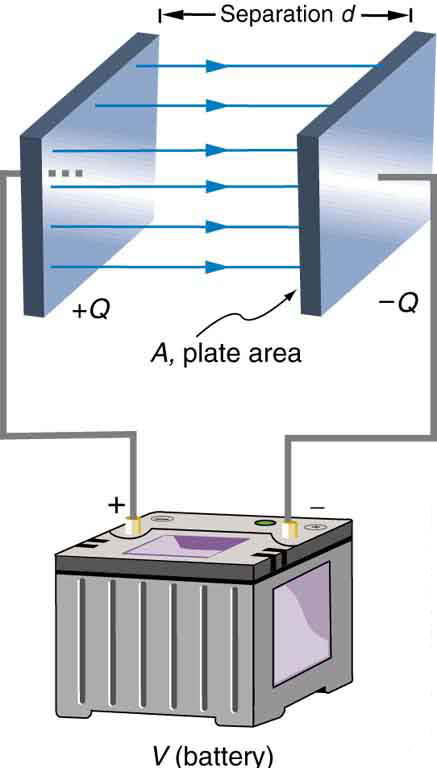
\includegraphics[width=4cm]{structure}
		\caption{The structure of a simple capacitor}
		\label{fig:structure}
	\end{figure}
	
	\subsection*{Concepts involving capacitors}
		\textbf{Capacitance} \newline
		Is the charge needed for each volt rise in the potential. In other words, it is how much charge can be stored within a given potential difference. That is,
		$$	C = \frac{Q}{V} $$
		Where:
		\begin{equation*}
			\begin{split}
				C = \text{Capacitance} \\
				Q = \text{Charge stored} \\
				V = \text{Potential difference/voltage between the plates}\\
			\end{split}
		\end{equation*}
		The SI unit of capacitance is called the Farad(in honor of Michael Faraday)
		, where 
		\begin{equation}
			1 F = \frac{1C}{1V}
		\end{equation}
	As we said earlier, capacitors are elements of circuits. Thus, we need special representation(symbols) for them so that we can know where they are located in circuits. In the diagram below, we see the representation of a capacitor in a circuit. Based on the type of capacitor it is, it might have different representations, but the first one will do for most of the topics we will be covering. 
	\begin{center}
		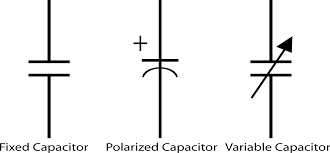
\includegraphics[scale=0.7]{cap.png}
		\label{fig:cap}
	\end{center}
    To understand how capacitors work, let's consider parallel plate capacitors. A system composed of two identical, parallel conducting plates separated by a distance is called a \textbf{parallel plate capacitor}. Look at Figure 1, to see the structure of parallel plate capacitors.
	\subsubsection*{Charging and Discharging Capacitors}
	We have discussed earlier on that capacitors act as batteries while discharging through circuit elements such as resistors or bulbs. The difference is, with capacitors this charging and discharging process takes a much smaller amount of time, than say a time it takes a battery to fully drain its stored energy. Let's for instance take a circuit that has a voltage source, a resistor and a capacitor. Assume the capacitor is charged to $V_0$ amount. When it is discharging, the initial current in the circuit is $\frac{V}{R}$(Recall Ohm's law), however, as time goes on, the potential differences decreases and as a result, the current also decreases. In capacitor terms, as time goes on, the potential difference(voltage) across the plates drops. When the current is higher(initially, since the voltage is higher), the capacitor empties really fast, but as time goes on, the current becomes lower and the capacitor also empties in a slower manner. \newline
	\begin{figure}[htp]
		\centering
		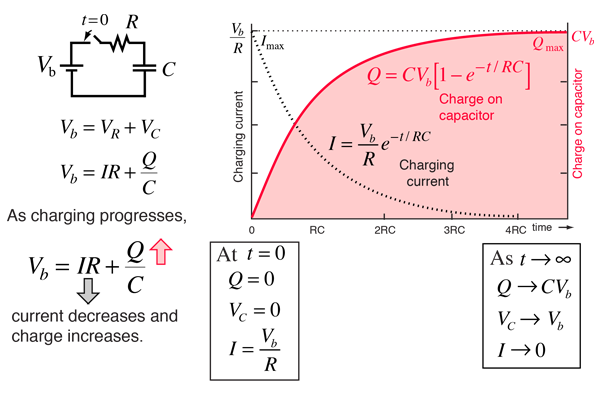
\includegraphics[width=9cm]{curve.png}
		\caption{Capacitor Charging Curve(Source: Hyperphysics)}
		\label{fig:charge}
	\end{figure} \newline \newline
	The time it takes for a capacitor to charge to its 63 percent of its intended amount during charging or to drop to 37 percent of its full amount during discharging is \textbf{RC} seconds. RC is called the time constant and is represented by the Greek letter Tau($\tau$)
	
	\subsection*{Factors Affecting Capacitance}
	A simple parallel plate capacitor contains parallel plates usually with an insulator in between them. The insulator in between the capacitors is called the \textbf{dielectric}. Capacitance can be affected by how much charge the plates can hold and the separation between them. Thus, the area of the plates(\textit{A}) and the separation between them(\textit{d}) are the main factors affecting the capacitance of a parallel plate capacitor.
	
		\begin{equation}
			C = \frac{\varepsilon_0A}{d}
		\end{equation}
		Where:
		\begin{itemize}
			\item $\varepsilon_0$ is a quantity called permitivitty of free space(vacuum) and it is the measure of the tendency of free space to be polarized. 
			\item A is the area of the plates.
			\item d is the separation distance between the plates
		\end{itemize}
	However, we have seen that we usually have an insulator(\textit{dielectric}) between the plates. When that happens, instead of $\varepsilon_0$(Permitivitty of free space), we have $\varepsilon$(Permitivitty of dielctric). Our equation, then, becomes:
	
			$$ C = \frac{\varepsilon A}{d}$$
		Where:
		\begin{itemize}
			\item $\varepsilon$ is the permitivitty of the dielectric.
		\end{itemize}    
		Permitivitty of a dielectric is related to the permitivitty of free space. The ratio between the permitivitty of a dielectric to that of free space is called \textbf{relative permitivitty} or \textbf{dielectric constant} and it is given by the Greek letter kappa($\kappa$).
			$$\kappa = \frac{\varepsilon}{\varepsilon_0}$$	
	\section*{Energy Stored in a capacitor}
	We have discussed previously that the use of capacitors is to store more charge at a lower potential(compared to other electrical equipments such as batteries.) When charges are stored on the plates of a capacitor, there is a potential energy that is stored in the capacitor as the plates are charged and are kept at a distance(think of the plates as point charges and a distance \textbf{r} between them). \\
	To find the energy stored in the capacitor, let's see how a capacitor's charge increases with respect to the voltage. \begin{center}
		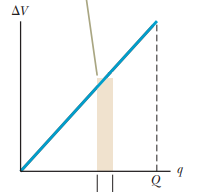
\includegraphics[scale=0.7]{v_q_curve.png}
	\end{center}
	We can see on the graph above that when a capacitor charges, the potential difference increases \textit{proportionally} with the charge being stored. When we have such situations, we take the average value of the charge. Since the charge is increasing with a constant slope, we take the midpoint of the line. \\
	That is,
	$$\frac{Q + 0}{2}$$
	That gives us the average value  of the charge while the potential difference on the plates of the capacitor reach the potential difference of the battery. If we look at the area under the curve of the \textbf{V} vs \textbf{Q} curve, we get the following:
	$$\text{Area}=\frac{1}{2}Q\times V$$
	The area under the line happens to be the energy stored in the capacitor. Thus,
	$$E = \frac{1}{2}Q\times V$$
	We can also express the area in terms of the capacitance and voltage.
	\\
	\newline
	We know that $$Q = C \times V$$
	That means,
	$$E = \frac{1}{2}(C\times V)\times V$$
	$$E = \frac{1}{2}CV^2$$
	
	\section*{Advanced: The meaning of the $\dfrac{1}{2}$}
	To understand the mathematical meaning of the $\frac{1}{2}$ at the beginning of the equation, we can make use of calculus and interested students can look at the following.(Remember how we used calculus to estimate the amount of charge left in a capacitor during discharge?)
	$$dW = \varDelta V\times dq$$
	$$dW = \frac{q}{C}\times dq$$
	To get the work, we integrate both sides:
	$$\int dW =\int_{0}^{Q}\frac{q}{C}dq$$
	$$ W =\frac{q^2}{2C}\Big|_0^Q $$
	$$ W =\frac{q^2}{2C}\Big|_0^Q $$
	$$ W =\frac{Q^2}{2C}$$
	Now, we can see how the $\frac{1}{2}$ has come to presence mathematically.
	\section*{Combination of Resistors}
	More often than not, we will use multiple capacitors in a circuit than just one. Thus, we have to compute the effective capacitance of the circuit.\newline
	We can combine the capacitors through a single path end-to-end with the same charges passing through them. This connection is called a \textbf{series} combination of capacitors. Look at the figure below for an example of a series combination of capacitors. \\
	\begin{center}
	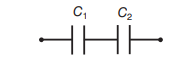
\includegraphics[scale=1]{series_capacitors.png}	
	\end{center}
	In both capacitors, we have the same charges flowing through them. Let the charge provided by the battery be \textbf{Q}, and if these capacitors are connected with series to the battery, a charge of \textbf{Q} passed through each of them. But, the potential difference provided by the battery is divided between the two capacitors. If the potential difference provided by the battery is \textbf{V}, we have the following: \newline
	$$V = V_1 + V_2$$
	We know that $V=\dfrac{Q}{C}$, thus,
	$$\dfrac{Q}{C} = \frac{Q_1}{C_1} + \frac{Q_2}{C_2}$$
	Since all the charges are equal,
	$$Q_1=Q_2=Q$$
	$$\frac{Q}{C} = \frac{Q}{C_1} + \frac{Q}{C_2}$$
	$$\frac{1}{C} = \frac{1}{C_1} + \frac{1}{C_2}$$    
	Thus, the reciprocal of the effective capacitance of the circuit is the reciprocal sum of each capacitance. Here, we can see that the effective capacitance can never be larger than the capacitance of each capacitance.
	In situations where the capacitors are connected in parallel(when the wire \textbf{branches} out), as in the figure below,\\
	\begin{center}
	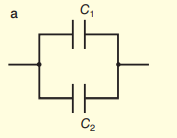
\includegraphics[scale=1]{parallel_capacitors.png}	
	\end{center}
	We have the potential difference to be the same for the capacitors connected in parallel. However, the charge from the battery is the sum of the charge in each capacitor.
	$$V = V_1 = V_2$$
	But we know that:
	$$Q=CV$$
	And
	$$Q = Q_1 + Q_2$$
	$$CV= C_1V_1 + C_2V_2$$
	$$CV = V(C_1+C_2)$$
	$$C = C_1 + C_2$$
	This means that the effective capacitance of capacitors connected in parallel. is the sum of each capacitance.
				
	
\end{document}